% Poster: Open-Source RAVEN and Embedder-Only Retrieval for Offline Robot Memory
% Compile with: pdflatex poster.tex (uses tikzposter)
% Size: 36" x 48" portrait. Adjust orientation= and paper= if needed.

\documentclass[25pt, a0paper, portrait, colspace=12mm, blockverticalspace=10mm]{tikzposter}
\usepackage[utf8]{inputenc}
\usepackage[T1]{fontenc}
\usepackage{lmodern}
\usepackage{amsmath, amssymb}
\usepackage{graphicx}
\usepackage{booktabs}
\usepackage{tabularx}
\usepackage{xcolor}
\usepackage{enumitem}
\usepackage{microtype}
\usetikzlibrary{arrows.meta, positioning, shapes.geometric, calc}

% --- Princeton color palette -------------------------------------------------
\definecolor{princetonOrange}{HTML}{E77500}
\definecolor{princetonOrangeLight}{HTML}{F5B870}
\definecolor{princetonBlack}{HTML}{1A1A1A}
\definecolor{princetonGrey}{HTML}{505050}
\definecolor{cardBg}{HTML}{FAFAFA}

% --- tikzposter theme ---
\definebackgroundstyle{plainWhite}{
  \draw[fill=white, draw=none] (bottomleft) rectangle (topright);
}
\definetitlestyle{titleBand}{
  width=\textwidth,
  roundedcorners=0,
  linewidth=0pt,
  innersep=12mm,
  titletotopverticalspace=0mm,
  titletoblockverticalspace=12mm,
}{
  \begin{scope}
    \draw[fill=princetonBlack, draw=none] (\titleposleft, \titleposbottom) rectangle (\titleposright, \titlepostop);
    \draw[fill=princetonOrange, draw=none] (\titleposleft, \titleposbottom) rectangle (\titleposright, \titleposbottom + 8mm);
  \end{scope}
}
\defineblockstyle{questionCard}{
  titlewidthscale=1.0, bodywidthscale=1.0, titleleft,
  titleoffsetx=0pt, titleoffsety=0pt,
  bodyoffsetx=0pt, bodyoffsety=0pt,
  bodyverticalshift=0mm,
  roundedcorners=4, linewidth=1pt,
  titleinnersep=8mm, bodyinnersep=10mm,
}{
  \draw[draw=princetonOrange, line width=1pt, fill=cardBg]
    (blockbody.south west) rectangle (blockbody.north east);
  \ifBlockHasTitle
    \draw[draw=none, fill=princetonOrange]
      (blocktitle.south west) rectangle (blocktitle.north east);
  \fi
}
\definenotestyle{plainNote}{
  targetoffsetx=0pt, targetoffsety=0pt,
  innersep=4mm, linewidth=1pt, roundedcorners=2,
}{
  \draw[draw=princetonGrey, fill=white, line width=1pt]
    (notebody.south west) rectangle (notebody.north east);
}

\definetheme{princetonPoster}{
  \usecolorpalette{Default}
  \usebackgroundstyle{plainWhite}
  \usetitlestyle{titleBand}
  \useblockstyle{questionCard}
  \usenotestyle{plainNote}
  \colorlet{titlefgcolor}{white}
  \colorlet{blocktitlebgcolor}{princetonOrange}
  \colorlet{blocktitlefgcolor}{white}
  \colorlet{blockbodybgcolor}{cardBg}
  \colorlet{blockbodyfgcolor}{princetonBlack}
}
\usetheme{princetonPoster}

% --- title -------------------------------------------------------------------
\title{\parbox{\linewidth}{\centering
  \color{white}\textbf{Open-Source RAVEN and Embedder-Only Retrieval for Offline Robot Memory}\\[6mm]
  {\Large\color{princetonOrangeLight}A DARPA TIAMAT Case Study}}}
\author{\color{white}Edison Zhu}
\institute{\color{white}Princeton University \quad\textbullet\quad Independent Work, 2026}

\begin{document}
\maketitle

% ============================================================================
% ROW 1 - Two columns, three blocks each
% ============================================================================
\begin{columns}

% ---- COLUMN 1 (left) ------------------------------------------------------
\column{0.5}

\block{How does a long-horizon robot remember what it has seen?}{
\large
Long-horizon robots need a memory that is \textbf{compact}, \textbf{grounded in space and time}, and \textbf{rich enough to preserve visual detail}.

\smallskip
Cloud LLMs aren't an option in the field. The challenge: build a memory pipeline that runs entirely offline, on commodity GPUs, without giving up navigation accuracy.
}

\block{What is RAVEN?}{
\large
RAVEN (Hu et al., RSS 2026) stores per-frame visual embeddings together with pose and timestamp in a vector database, then uses a VLM agent to retrieve and reason iteratively.

\smallskip
\textbf{Four retrieval tools:}
\begin{itemize}[leftmargin=*, itemsep=2pt]
  \item Text-based --- VLM-proposed query embedding
  \item Image-based --- visual nearest neighbor
  \item Time-based --- $K$ consecutive frames from a timestamp
  \item Position-based --- $K$-NN over agent poses
\end{itemize}

\smallskip
The agent loops until it has enough evidence to emit an answer (text, position, or timestamp).
}

\block{Can RAVEN run without the cloud?}{
\large
The paper's headline numbers use cloud VLMs (Gemini~2.5/3, GPT-5.2). The authors note that medium-sized open VLMs can underperform an embedder-only baseline (\S5.3).

\smallskip
\textbf{We test the offline configuration} on DARPA TIAMAT data:
\begin{itemize}[leftmargin=*, itemsep=2pt]
  \item Local open-source VLMs (Gemma, Qwen) via Ollama
  \item Four visual embedders compared as a no-LLM baseline
\end{itemize}
}

\block{How did we test?}{
\large
546 egocentric frames (\(\sim\)7.5 min) through an indoor Habitat residence: entry, living, kitchen, bath, and dining.

\smallskip
\centering
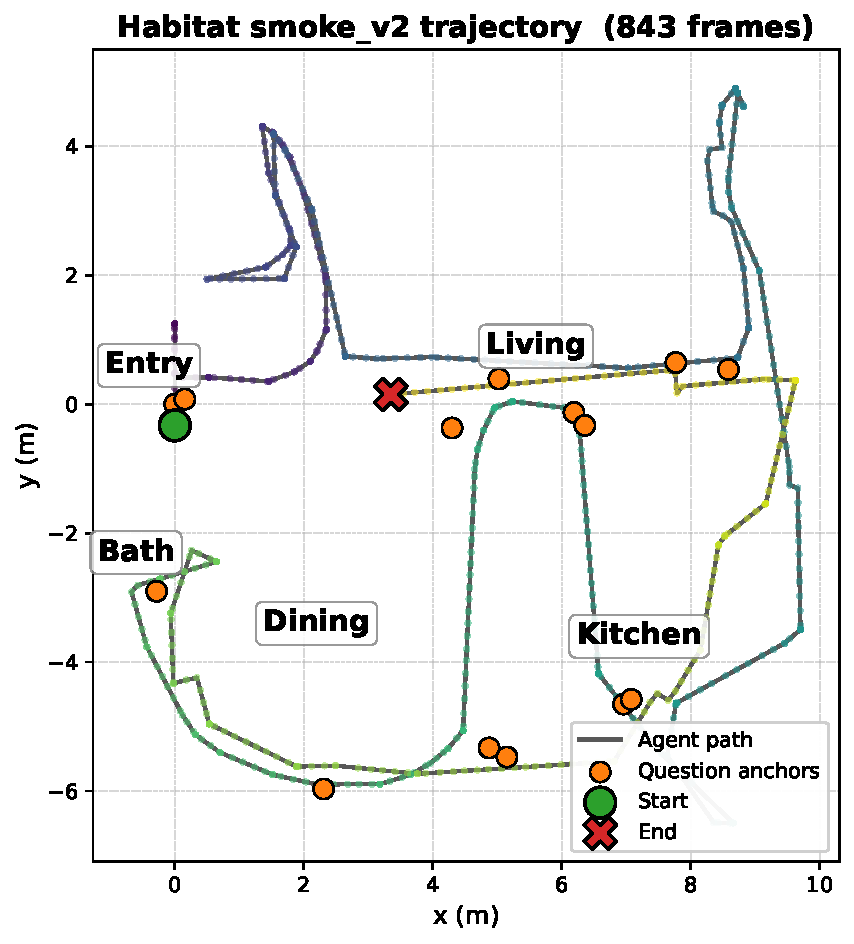
\includegraphics[width=0.9\linewidth]{figures/scene_minimap.pdf}

\medskip
\raggedright
We authored a \textbf{20-question, five-level suite} over the trajectory. Each level isolates a different capability, so we can pinpoint \emph{where} on the difficulty curve the LLM stops being optional.

\smallskip
\begin{tabularx}{\linewidth}{lX}
\textbf{L1 Direct}      & ``Where is the purple chair?'' \\
\textbf{L2 Indirect}    & ``Where can I sit comfortably?'' \\
\textbf{L3 Spatial}     & ``Closest room to the entry?'' \\
\textbf{L4 Multi-step}  & ``Where did the agent start?'' \\
\textbf{L5 Negation}    & ``Chair NOT in the kitchen?'' \\
\end{tabularx}

\smallskip
Multi-position ground truth (2--3 acceptable poses per question) lets us grade ``right room, wrong pose'' separately from ``wrong room entirely.''
}

% ---- COLUMN 2 (right) -----------------------------------------------------
\column{0.5}

\block{Which embedders and VLMs did we compare?}{
\large
\textbf{Embedders (4):}
\begin{itemize}[leftmargin=*, itemsep=2pt]
  \item QQMM-v2 \hfill 3584d (RAVEN's pick)
  \item CLIP ViT-L-14 \hfill 768d \quad (OpenAI 2021)
  \item CLIP ViT-H-14 \hfill 1024d \quad (LAION-2B)
  \item SigLIP-384 \hfill 1152d \quad (WebLI)
\end{itemize}

\smallskip
\textbf{Open VLMs via Ollama:} Gemma~3 12B/27B, Gemma~4 26B/31B, Qwen2.5-VL 3B/32B (4-bit), Qwen3-VL 32B (4-bit).
}

\block{How did we grade?}{
\large
The camera stands back to \emph{see} objects, so a correct retrieval is naturally 2--4\,m from the object's pose. We use a \textbf{viewing-distance-aware metric}:

\medskip
\centering
\begin{tabular}{ll}
\toprule
\textbf{Bucket} & \textbf{Distance to nearest GT} \\
\midrule
Strict & $d \leq 3.5$\,m \\
Semi   & $3.5 < d \leq 5.5$\,m \\
Wrong  & $d > 5.5$\,m \\
\bottomrule
\end{tabular}

\medskip
\raggedright
For \emph{camera-pose} queries (L4.3, L5.4 --- ``where the agent stood'') we use the tighter $\leq$1.5\,m / $\leq$3.0\,m thresholds.
}

\end{columns}

% ============================================================================
% ROW 2 - Results across full width via columns of 1
% ============================================================================
\begin{columns}

\column{0.5}

\block{Is bigger always better?}{
\centering
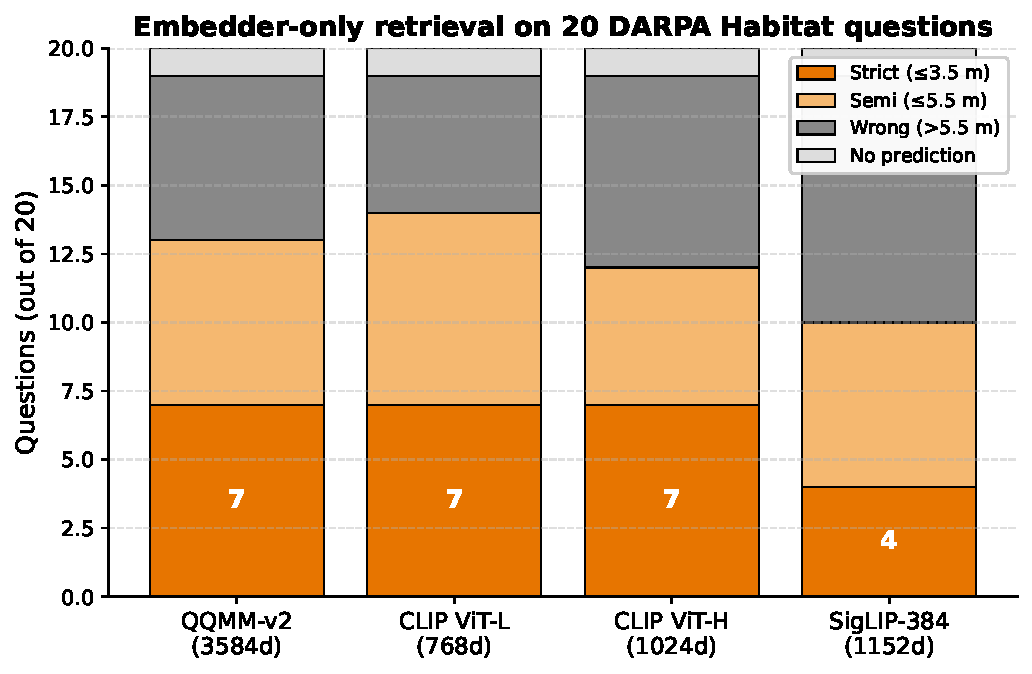
\includegraphics[width=0.98\linewidth]{figures/headline_bars.pdf}

\medskip
\raggedright\large
\textbf{No.} A 768-dim CLIP from 2021 ties a 3584-dim navigation-specialized QQMM-v2 on strict accuracy (7/19 each) and \emph{wins} on mean distance (3.71\,m vs 5.20\,m). SigLIP-384 lags despite a comparable parameter count.
}

\column{0.5}

\block{When is a VLM agent needed?}{
\centering
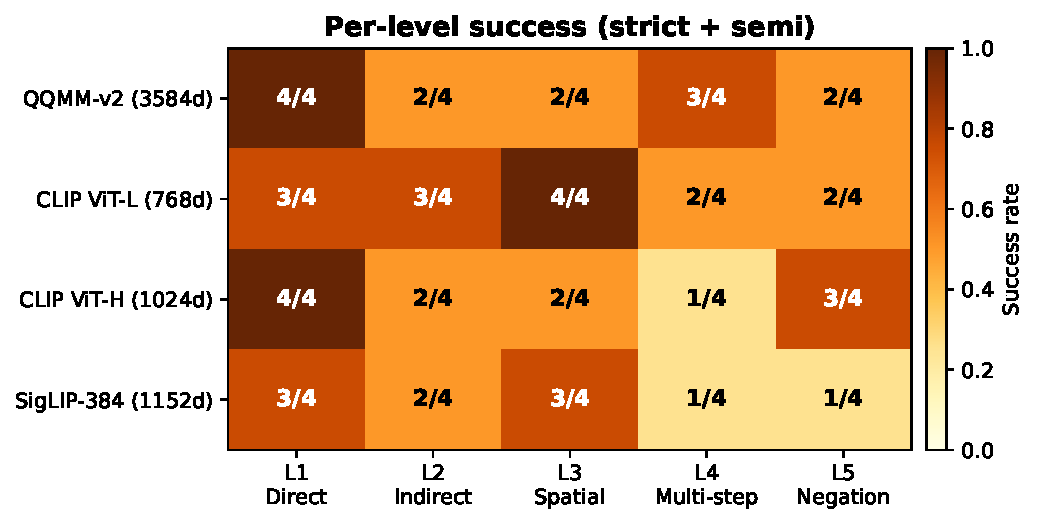
\includegraphics[width=0.98\linewidth]{figures/per_level_heatmap.pdf}

\medskip
\raggedright\large
\textbf{Only on L3--L5.} Embedder alone clears L1/L2 at $\geq$75\%; adding an agent here is wasted compute. On L3--L5, the embedder never breaks 50\%, so the agent earns its cost by composing multiple retrievals.

\medskip
\textbf{Conclusion.} The retriever sets what is \emph{findable}; the agent sets what is \emph{answerable}. \textbf{Embedder-only} (QQMM) plateaus at \textbf{42.1\%} --- a nearest-neighbor lookup cannot compose, negate, or reason spatially. \textbf{Embedder+agent} (QQMM\,$+$\,tool-using VLM) reaches \textbf{81.6\%} on the same 19 questions, with the full $+40$\,pp concentrated on L3 spatial ($+75$\,pp), L4 multi-step ($+38$\,pp), and L5 negation ($+37$\,pp).

\medskip
\textbf{Takeaway.} Spend the embedder budget on the strongest open model you can run locally; spend the agent budget only when the question requires composition.
}

\end{columns}

% ============================================================================
% ROW 3 - Failure modes and fixes
% ============================================================================
\begin{columns}

\column{0.5}

\block{Where does open-VLM RAVEN fail?}{
\large
\begin{itemize}[leftmargin=*, itemsep=4pt]
  \item \textbf{Retrieval loops.} The same query is re-issued 4--6$\times$ when top-$K$ doesn't help (\texttt{"coffee machine"} 6$\times$, \texttt{"entryway"} 6$\times$).
  \item \textbf{Prose without coordinates.} L3.1 / L3.3 return the correct room name (``the entryway'', ``the living room'') but no $(x, y, z)$ --- a coordinate-plumbing gap, not a reasoning failure.
  \item \textbf{Right frame, wrong coordinate.} Top-$K$ retrieval lands on the correct frame but the reported pose drifts from ground truth.
  \item \textbf{Under-used non-text retrievers.} Only \textbf{1/20} queries triggered the time- or position-based retriever.
\end{itemize}
}

\column{0.5}

\block{What can we fix without retraining?}{
\large
\begin{enumerate}[leftmargin=*, itemsep=4pt]
  \item \textbf{Diversify queries.} After $K$ identical retrievals, force a prompt-level rewrite of the query before re-issuing.
  \item \textbf{Coordinate fallback.} When the VLM returns a room name with no coordinate, emit the centroid of the retrieved frames' poses. This salvages every observed L3 failure.
  \item \textbf{Tool-use priming.} Add few-shot exemplars showing the time and position retrievers being called after text retrieval fails.
\end{enumerate}

\medskip
None require fine-tuning. None touch the retrieval substrate.
}

\end{columns}

% ============================================================================
% ROW 3.5 - Future: jointly integrate the four changes
% ============================================================================
\block{What's next: route easy queries around the VLM \emph{and} fix the agent path together}{
\begin{minipage}[c]{0.52\linewidth}
\centering
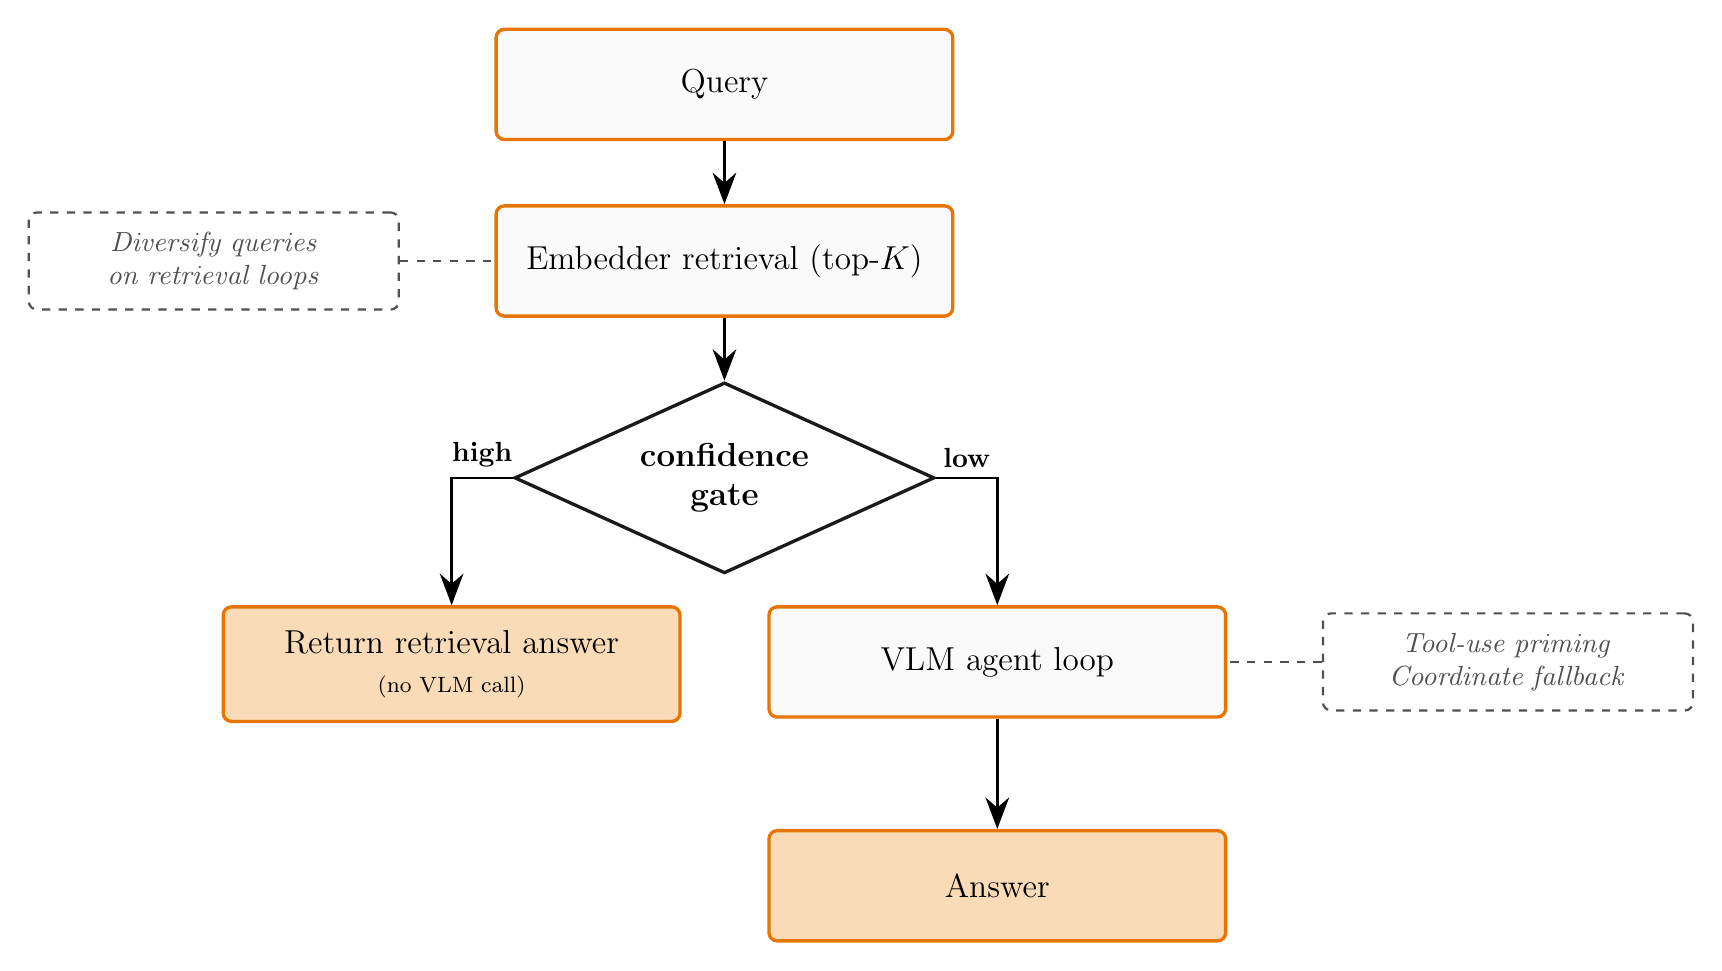
\begin{tikzpicture}[
  every node/.style={font=\large},
  box/.style={draw=princetonOrange, line width=1.2pt, fill=cardBg, rounded corners=3pt,
              minimum height=14mm, minimum width=58mm, align=center, inner sep=3mm},
  decision/.style={draw=princetonBlack, line width=1.2pt, fill=white, diamond, aspect=2.2,
                   align=center, inner sep=2mm, font=\large\bfseries},
  fix/.style={draw=princetonGrey, line width=0.8pt, dashed, fill=white, rounded corners=3pt,
              align=center, inner sep=2.5mm, font=\normalsize\itshape, text=princetonGrey},
  arrow/.style={-{Stealth[length=4mm]}, line width=1pt},
  fixarrow/.style={dashed, line width=0.7pt, draw=princetonGrey},
  node distance=8mm and 14mm
]
\node[box] (q) {Query};
\node[box, below=of q] (emb) {Embedder retrieval (top-$K$)};
\node[decision, below=of emb] (gate) {confidence \\ gate};
\node[box, below left=10mm and -8mm of gate, fill=princetonOrangeLight!50] (ans1) {Return retrieval answer \\ \footnotesize (no VLM call)};
\node[box, below right=10mm and -8mm of gate] (vlm) {VLM agent loop};
\node[box, below=14mm of vlm, fill=princetonOrangeLight!50] (ans2) {Answer};

\draw[arrow] (q) -- (emb);
\draw[arrow] (emb) -- (gate);
\draw[arrow] (gate.west) -| node[near start, above, font=\normalsize\bfseries]{high} (ans1.north);
\draw[arrow] (gate.east) -| node[near start, above, font=\normalsize\bfseries]{low} (vlm.north);
\draw[arrow] (vlm) -- (ans2);

\node[fix, left=12mm of emb, text width=42mm] (f1) {Diversify queries \\ on retrieval loops};
\node[fix, right=12mm of vlm, text width=42mm] (f2) {Tool-use priming \\ Coordinate fallback};
\draw[fixarrow] (f1.east) -- (emb.west);
\draw[fixarrow] (f2.west) -- (vlm.east);
\end{tikzpicture}
\end{minipage}%
\hfill
\begin{minipage}[c]{0.44\linewidth}
\large
A confidence gate on the retriever short-circuits L1/L2 queries before the VLM is ever called, while L3--L5 still get the full agent loop --- now augmented with the three prompt-level fixes wired into the same path.

\medskip
The four changes \textbf{interact}: coordinate fallback shortens the path the gate is trying to avoid; query diversification reshapes what counts as ``high confidence''; tool-use priming changes which queries are actually reasoning-required.

\medskip
\textbf{Add them jointly, not as disjoint patches} --- evaluating them together on the same suite is the only way to measure their combined lift.
\end{minipage}
}

% ============================================================================
% ROW 4 - Bottom verdict (full width)
% ============================================================================
\block{Can you run RAVEN offline?}{
\large\centering
\textbf{Yes.} Use embedder-only retrieval for L1/L2 queries (no LLM cost, no internet). Use a local open-source VLM with the three prompt-level fixes for L3--L5. No cloud, no retraining, no specialized hardware beyond a single L40 GPU pair.
}

% ============================================================================
% References + contact (full width, two columns)
% ============================================================================
\begin{columns}
\column{0.72}
\block{References}{
\small
\begin{enumerate}[leftmargin=6mm, itemsep=1pt, label={[\arabic*]}]
  \item Y.~Hu, Z.~Zheng, L.~Zha, C.~Xing, R.~Singh, O.~Hossain, A.~Loquercio, D.~Shah. \textbf{RAVEN}: Long-Horizon Reasoning and Navigation with a Visuo-Spatial-Temporal Memory. \emph{RSS}, 2026.
  \item A.~Anwar et al. \textbf{ReMEmbR}: Building and Reasoning Over Long-Horizon Spatio-Temporal Memory for Robot Navigation. 2024.
  \item A.~Radford et al. Learning Transferable Visual Models from Natural Language Supervision (\textbf{CLIP}). \emph{ICML}, 2021.
  \item X.~Zhai et al. Sigmoid Loss for Language-Image Pre-training (\textbf{SigLIP}). \emph{ICCV}, 2023.
  \item Z.~Xue et al. \textbf{QQMM-embed-v2}. \texttt{huggingface.co/youzexue/QQMM-embed-v2}, 2025.
  \item J.~Johnson, M.~Douze, H.~J\'egou. Billion-scale similarity search with GPUs (\textbf{FAISS}). \emph{IEEE TBD}, 2019.
  \item Habitat-Sim / Habitat AI Challenge. \texttt{aihabitat.org}.
  \item DARPA \textbf{TIAMAT} Program documentation, 2025.
  \item JIRL (UPenn). \textbf{DARPA TIAMAT Competition Code}. \texttt{github.com/Jirl-upenn/darpa-tiamat-competition-code}, 2025.
\end{enumerate}
}
\column{0.28}
\block{Contact \& code}{
\large
Edison Zhu \\
\texttt{ezhu@princeton.edu} \\[2mm]
Princeton University \\
Independent Work, 2026 \\[3mm]
Advisor: \emph{[advisor name]}
}
\end{columns}

\end{document}
